% chap3.tex
%

\mychapter{Structured and Unstructured Data for Factoid Question Answering}
\label{chapter:factoid}

\noindent

There are multiple ways to marry unstructured and structured data for joint question answering: convert structured data to unstructured format or vice versa, convert all data to certain intermediate representation or to leave them as is and link the data sources.
In my thesis I focus on two approaches: relation extraction for knowledge base completion, and semantic annotation of text for hybrid question answering.

\section{Relation Extraction for Knowledge Base Completion}
\label{sec:relation_extraction}

The information on the web is stored in multiple different forms, such as natural language statements, tables and infoboxes, images \etc.
In this work I focus on yet another source of information: question-answer pairs.
Community question answering archives contain hundreds of millions of question and corresponding answers.
Information expressed in these pairs might be hard to extract or not exist at all in other formats.

\subsection{Relation extraction from Question-Answer pairs}
\label{subsec:cqa_relextract}

PUT SUMMARY OF MY NAACL STUDENT RESEARCH WORKSHOP PAPER.

% BELOW IS MY ANOTHER IDEA, BUT IT'S VAGUE AND DOESN'T HAVE ANY CONCRETE PLAN
% \subsection{Question-guided relation extraction}
%\label{subsec:question_based_relextract}
%The idea is that we can aggregate related questions and relation extraction patterns.
%When a person asks a question, we retrieve passages and sentences to extract the answer from.
%Imaging a question is asking a certain property of an entity.
%If we can retrieve a sentence, that mentions this entity along with a candidate answer, we can build a pattern for relation extraction.
%This pattern will be connected to the question ``template''.
%Likewise, if we already have relation extraction patterns we can boost those that are retrieve in response to the question and save this connection.

%Hypothesis:
%\begin{enumerate}
%\item Patterns retrieved in response to the question are better in quality, we can boost them. We can try to verify this on some relation extraction dataset and questions from some query log. We can also try to use some KBQA dataset.
%\item Patterns mined for questions should help question answering. This is essentially weak supervision for training knowledge base question answering using text based question answering.
%\end{enumerate}

%Problems:
%\begin{itemize}
%\item How to extract new predicates? If we have a question, and a sentence is mentioning a pair of non-related entities, how can we make a new one?
%\item How to deal with more complex questions, that are not simple relations
%\end{itemize}

%Useful dataset: MSN query log, SimpleQuestions from Facebook, WebQuestions, NYT relation extraction dataset.

%This approach can also be applied to open IE.
%There are sentence selection methods for question answering.
%We can extract noun phrases (NP mentioned in question and supposedly answer NP), and then aggregate all sentences, that mention the same NPs together.
%Hypothesis is, that we can extract patterns, that will answer the same question for other entities.

\section{Semantic Text Annotations for Hybrid Question Answering}
\label{sec:text+kb}

Converting unstructured information into structured form by extracting knowledge from text suffers from certain quality losses.
Existing relation extraction tools aren't perfect, in particular due to recall losses a lot of information is left behind.
Moreover, extractions contain certain level of incorrect information due to precision losses.
These errors cap the upper bound on the question answering system performance.

Here I propose to utilize the synergy of structured and unstructured data, and exploit the advantages of each of them to overcome the limitations of the other.
More particularly, I propose to annotate and index mentions of knowledge base entities in text documents.
Such a representation induces a special kinds of edges to the knowledge base, and allows one to traverse this edges in both directions.
These links open up many opportunities for QA reasoning, \eg retrieving all the information about the entity by going from a mention to a KB entity, finding relations between entities by retrieving text passages that mention both of them, extracting candidate evidence by retrieving passages that mention question and answer entities along with some question terms, and so on.

--- THE NEXT PIECE IS OLDER, NEED TO REVIEW

Question answering from text corpora typically starts by retrieving a set of potentially relevant documents using the question (or some transformation of the question \cite{AgichteinLG01}) as the query, and then extracting entities, phrases, sentences or paragraphs believed to be the answer to the question.
However, the information available in the retrieved pieces of text is very limited and often not enough to decide whether it can be the answer to the given question.
For example, below is one of the questions from TREC QA 2007 dataset:\\
\textit{``What republican senators supported the nomination of Harriet Miers to the Supreme Court?''}\\
A candidate answer sentence \textit{``Minority Leader Harry Reid had already offered his open support for Miers.''} mentions a senator ``Harry Reid'' and clearly says about his support of the nomination.
However, ``Harry Reid'' is not a correct answer to the question because he is a member of the Democratic party.
This information is not available in the answer candidate sentence, but it is present as one of the properties in Freebase: [Harry Reid, political\_party, Democratic party]\footnote{Actually, in Freebase the entities are connected by a path of length 2 through a mediator node. The predicates on the path are: /government/politician/party and /government/political\_party\_tenure/party}.
Therefore, by looking into the knowledge available about the mentioned entities a QA system can make a better judgment about the candidate answer.

% THIS IS THE CORRESPONDING PIECE ON KBQA, I DON'T REALLY LIKE IT

% Question answering over linked data (knowledge bases) converts a natural language question into a structured query, such as SPARQL.
%The main challenge for such systems is to map words and phrases from the question to the corresponding entities and predicates from a KB.
%Usually, such lexicon is built during training using ground truth question-query pairs \cite{CaiY13} or question-answer pairs \cite{BerantCFL13:sempre}.
%Improvements were made by extending the lexicon using Wikipedia and patterns expressing certain predicates obtained via distant supervision \cite{bastmore:cikm:2015:aquu,BordesCW14:emnlp,ReddyLS14,yih:ACL:2015:STAGG,YaoD14}.
%But still, the amount of available labeled or weakly labeled training data is much smaller than the amount of unstructured data.
%This unstructured data will complement the learned lexicon, e.g. even if a question about a certain predicate wasn't seen during training, a set of text paragraphs mentioning both of the related entities can provide a QA system with enough evidence to make the correct decision.

----

\subsection{Approach}
\label{subsec:text+kb_approach}

\begin{figure*}
\centering
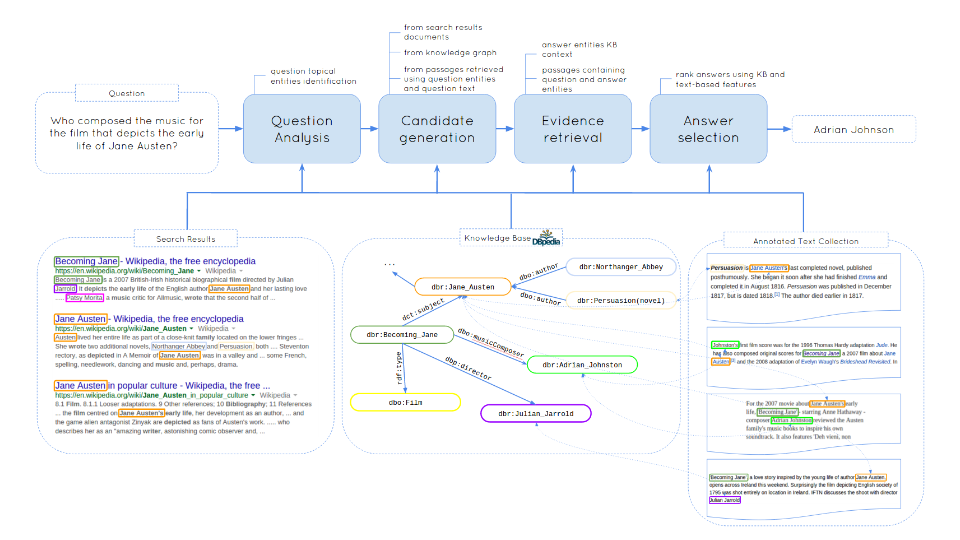
\includegraphics[width=\textwidth]{img/text_and_kb}
\caption{Architecture of a hybrid factoid question answering system, that uses a combination of structured knowledge base and unstructured text data}
\label{fig:text_kb}
\end{figure*}

The architecture of the hybrid QA model I propose is presented on Figure \ref{fig:text_kb}.
Here are the main stages of the question answering process:
\begin{itemize}
\setlength\itemsep{0em}
\item \textbf{Pre-processing}: identify mentions of KB entities in text document collection and index the documents text and mentions in separate fields
\item \textbf{Topical entity identification}: search the text collection using question (or reformulated question \cite{AgichteinLG01}) as a query and use an approach similar to \cite{cornolti2014smaph} to detect question topical entities
\item \textbf{Candidate generation from text}: extract candidate answer (or intermediate answer) entities with evidence from the retrieved text documents using existing techniques, e.g. \cite{tsai2015web}.
\item \textbf{Candidate generation from KB}: explore the KB neighborhood of question topical entities and entities extracted from text documents on the previous step
\item \textbf{Candidate generation from KB \& Text}: use entity and text index to find entities mentioned near question topical entity and question terms in the document collection
\item \textbf{KB evidence extraction}: match neighborhood of answer entities (entity type and other entities) against the question to get additional evidence
\item \textbf{Text evidence extraction}: estimate the similarity between the collection text fragments mentioning question and answer entities and the question text
\item \textbf{Rank candidate}: rank candidate answers using evidence extracted from the KB as well as from text
\end{itemize}

Let's consider an example question ``\textit{Who composed the music for the film that depicted the early life of Jane Austen?}'' from the QALD dataset\footnote{http://greententacle.techfak.uni-bielefeld.de/~cunger/qald/} (Figure \ref{fig:text_kb}).
Even though it's quite easy to identify the ``\texttt{Jane Austen}'' entity in the question, the knowledge base (dbPedia in this example) cannot help us to determine which movie is being referred to.
However, there are a lot of documents on the web, that do mention the ``\texttt{Becoming Jane}'' movie and say what is it about.
Unfortunately, extracting the name of the composer from these documents is quite challenging, but this task can be easily accomplished by checking the value of the \texttt{musicComposer} property in the knowledge base.
At the end, for each candidate answer entity, we have all the KB information and passages that mention this entity as evidence to help with the correct answer selection.

\subsection{Evaluation}
\label{sec:factoid_evaluation}

\subsubsection{Knowledge base QA}

I THINK HERE WE CAN INCLUDE OUR RESULTS ON TEXT2KB.

Most of the recent work on knowledge base question answering and semantic parsing have been evaluated on the WebQuestions dataset \cite{BerantCFL13:sempre}, which contains a collection of question text and correct answer entities.
The questions were collected using Google Suggest API and answers crowdsourced using Amazon Mechanical Turk\footnote{http://mturk.com/}
The proposed approach will be compared against the previous results\footnote{http://goo.gl/sePBja} on this dataset.
Again, web can be used as a text collection which can be queried using Bing Search API.
Relation extraction patterns can be mined using distant supervision from ClueWeb collection using publicly available dataset of Freebase annotations \cite{gabrilovich2013facc1}.

\textbf{New factoid question answering dataset}.
However, WebQuestions dataset has certain limitations, e.g. questions mined using Google Suggest API have very similar structure and lexicon, and to find the answer to the mined questions users were asked to use the question entity Freebase profile page,  which only include entities connected directly with a predicate or through a mediator node.
Therefore most of the state-of-the-art results on the dataset use a small number of predefined logical form patterns.
On the other hand CQA websites have a fraction of factoid questions with provided text answers.
Here I propose to use to construct a new dataset for question answering over Freebase by selecting a subset of QnA pairs with at least one entity in question and answer and some reasonable filtering heuristics and manual validation using crowdsourcing (e.g. through Amazon Mechanical Turk).
Existing systems need to be retrained and tested on the new dataset to compare against the proposed model.

\subsubsection{Text-based QA}

WE WILL ANNOTATE TREC DATASETS WITH ENTITIES!!!!

TREC QA datasets served as a benchmark for various question answering systems.
Therefore, to evaluate the proposed approach for question answering over text enriched with the structured data I propose to test it on dataset derived from TREC QA and compare against existing strong baselines, including the most related approaches \cite{Fader:2014:OQA:2623330.2623677,Sun:2015:ODQ:2736277.2741651}.
The proposed system can use the web as the corpus and query it using Bing Search API\footnote{https://datamarket.azure.com/dataset/bing/searchweb}.
Freebase and Reverb extractions \cite{FaderSE11} are examples of schema-based and open knowledge bases that can be used for the experiments.
The metrics used for evaluation typically include accuracy and mean reciprocal rank (MRR).

For non-factoid question answering this year TREC pioneered a new question answering track - TREC LiveQA\footnote{http://trec-liveqa.org/}, which targets questions asked by real users of Yahoo! Answers website.
This year the deadline for system submission was on August 31 and my system trained on CQA QnA pairs participated in the challenge.
The results will be available on the TREC Conference in November 2015.
Organizers plan to continue with another TREC LiveQA task next year and this is going to be a good estimation of the effectiveness of the proposed techniques on hard real user questions.


\section{Summary}
In this section we considered two different ways of combining unstructured and structured data to improve factoid question answering.
Relation extraction from question-answer pairs aims at filling some gaps in KB fact coverage, whereas semantic annotations of text documents provides a way to incorporate information available in unstructured text documents for reasoning along with KB data to improve the performance of factoid question answering.

Factoid questions represent just a part of user information needs. Many problems require more elaborate response, such as a sentence, list of instructions or in general a passage of text.
Such questions are usually referred to as non-factoid questions and they will be the focus of the next Chapter.

\clearpage